\documentclass[12pt,a4paper]{article}
\usepackage{fontspec}
\usepackage{amsmath}
\usepackage{amssymb}
\usepackage{bm}
\usepackage{tikz}
\setmainfont{Adobe Kaiti Std}
\thispagestyle{empty}
\pagestyle{empty}
\begin{document}

\fancyfoot[C]{by chinasjtu@msn.com }

\newcommand{\nl}{\newline}

\newcommand{\ntinf}{\lim\limits_{n \to \infty}}
\newcommand{\xtinf}{\lim\limits_{x \to \infty}}

\newcommand{\Atinf}{\lim\limits_{A \to \infty}}
\newcommand{\Rtinf}{\lim\limits_{R \to \infty}}

\newcommand{\ntx}[1]{\lim\limits_{n \to #1}}
\newcommand{\xtx}[1]{\lim\limits_{x \to #1}}
\newcommand{\ttx}[1]{\lim\limits_{t \to #1}} 
\newcommand{\ktx}[1]{\lim\limits_{k \to #1}} 
\newcommand{\dxtx}[1]{\lim\limits_{\Delta x \to #1}}

\newcommand{\jfab}{\int_{a}^{b}}
\newcommand{\jf}[2]{\int_{#1}^{#2}}

\newcommand{\nsum}[2]{\sum\limits_{n=#1}^{#2}}
\newcommand{\isum}[2]{\sum\limits_{i=#1}^{#2}}
\newcommand{\ksum}[2]{\sum\limits_{k=#1}^{#2}}

\newcommand{\nsuminf} {\nsum{1}{\infty}}
\newcommand{\ksuminf} {\ksum{1}{\infty}}
\newcommand{\isuminf} {\isum{1}{\infty}}





第7章 定积分

$7.1.定积分概念与可积性条件$

$记法:T \subset [a,b],对[a,b]的分法T,a=x_0<x_1<...x_n=b$

$\{\zeta_k\}在分法下对[x_{k-1},x_k]中点\zeta_k的取法k=1~n$

$\delta(f,T,\zeta)对T \subset [a,b]以及\{\zeta_k\}作\sum\limits_{i=1}^n f(\zeta_k)\Delta x_k (Riemann和) $

$ex:\int_{a}^{b}\frac{1}{x^2}dx (1)取\zeta_n=\sqrt{x_nx_{n-1}} 3种方法$

$(2)x_n=ar^n,r=\sqrt[n]{\frac{b}{a}},取\zeta_n=x_{n-1}$

$(3)利用中值定理,取成中值定理中的\zeta_k$

$\nl$

$例:设f(x)g(x) \in C[a,b],证明$

$\lim_{\lambda \to 0} \sum\limits_{k=1}^n f(\zeta_k)g(\theta_k)\Delta x_k=\int_{a}^{b}f(x)g(x)dx$

$其中\zeta_k \theta_k \in [x_{k-1},x_k],k=1~n,对\forall T \subset [a,b],\forall \{\zeta_k\}\{\theta_k\}$

$Darboux和:T' \supset T,在分法T中添加分点,成为加细分法T'$

$T=T_1 \cup T_2,旧分法T_1和T_2的所有分点合成加旧分法T$

$\nl$

$性质1,对\forall T \subset [a,b],\forall \{\zeta_k\}有$

$m(T) \le \delta(f,T,\zeta) \le M(T)$

$inf \delta (f,T,\zeta) = m(T),sup \delta (f,T,\zeta) = M(T)$

$若添加k个分点,0 \le M(T)-m(T) \le k(M-m)\lambda$

$称sup_T\{s(T)\}为f(x)在[a,b]上的下积分,记为\underline{\int_{a}^{b}}f(x)dx$

$称inf_T\{s(T)\}为f(x)在[a,b]上的上积分,记为\overline{\int_{a}^{b}}f(x)dx$

$Darboux定理:\lim_{\lambda \to 0}S(T)=\underline{\int_{a}^{b}}f(x)dx,\lim_{\lambda \to 0}s(T)=\overline{\int_{a}^{b}}f(x)dx$

$证明:\forall \epsilon >0,由inf_T\{s(T)\}=\overline{\int_{a}^{b}}f(x)dx定义可知$

$\exists T' \subset [a,b],S(T')<\overline{\int_{a}^{b}}f(x)dx+ \frac{\epsilon}{2}$

$设T'共有k个分点,则\forall T \subset [a,b],则T \cup T'比T至多多k个分点$

$S(T)-S(T \cup T') \le k(M-m)\lambda$

$S(T) \le S(T \cup T')+k(M-m)\lambda \le S(T')+k(M-m)\lambda$

$取\delta = \frac{\epsilon}{2(M-m)},当\lambda < \delta 时,有S(T) \le \int_{a}^{b}f(x)+\epsilon$

$又因S(T) \ge \underline{\int_{a}^{b}}f(x)dx > \underline{\int_{a}^{b}}f(x)dx-\epsilon$

$故|S(T)-\underline{\int_{a}^{b}}f(x)dx| < \epsilon$

$\forall \epsilon>0,\exists \delta>0,|\delta(f,T,\zeta)| < \epsilon,\forall T,\lambda < \delta$

$故|s(T)-I| \le \epsilon, |S(T)-I| \le \epsilon$

$I-\epsilon \le s(T) \le S(T) \le I+\epsilon$

$0 \le \overline{\int_{a}^{b}}f(x)dx - \underline{\int_{a}^{b}}f(x)dx \le S(T)-s(T) \le 2 \epsilon$

$由\epsilon 任意性,即有\overline{\int_{a}^{b}}f(x)dx = \underline{\int_{a}^{b}}f(x)dx$

$\nl$

$T'' = \sum\limits_{k''}\omega_{k''} \Delta x_{k''} < \frac{\epsilon}{2}$

$T' = \sum\limits_{k'}\omega_{k'} \Delta x_{k'} < M\sum\limits_{k'}\Delta_{k'}< M \frac{\epsilon}{2M}$

$\nl$

$例:f(x) \in R[a,b],f(x) \ge m > 0,x \in [a,b),证\frac{1}{f(x)} \in R$

$依题意有\forall \epsilon > 0, \exists T \subset [a,b], \sum\limits_{k=1}^{n}\omega_k \Delta x_k < \epsilon$

$设\omega_{k'}=sup\{|\frac{1}{f(x')}-\frac{1}{f(x'')}|\}$

$因为|\frac{1}{f(x')}-\frac{1}{f(x'')}| \le \frac{1}{m^2} |f(x')-f(x'')|,....$

$\nl$
$\int_{a}^{b}|f(x)|dx必须分段讨论$

$原函数F'(x)=f(x) \forall x \in I$

$可积函数 \exists I \in R,\forall \epsilon >0,\exists \delta >0,|s(f,T,\zeta)|< \epsilon,\forall T,\zeta, \lambda < \delta$

$例:F(x)=\begin{cases} x^2sin\frac{1}{x},1 \ge x >0,\\ 0,x=0 \end{cases},但F'(x)不可积$

$无穷间断点,非单调,必不可积? \frac{1}{x}-[\frac{1}{x}]可积$

$\nl$
$预备命题1.Schwarg不等式,对\forall a_k,b_k (k=1\sim n)有$

$(\sum\limits_{k=1}^{n}a_kb_k)^2 \le (|\sum\limits_{k=1}^{n}a_kb_k|)^2 \le (\sum\limits_{k=1}^{n}a_k^2)(\sum\limits_{k=1}^{n}b_k^2)$

$\nl$
$预备命题2:设f(x)在区间上有界,若sup_I\{f^2(x)\}=\beta^2$
$则有sup\{|f(x)|\}=\beta (\beta \ge 0)$

$
习题:均可积
\begin{cases}
f(x)=\begin{cases}0,x \ne 0 \\ 1,x=0 \end{cases} \\
g(x)=Riemamm函数
\end{cases}
f(g(x))不可积
$

$不可积函数对于特定T,\zeta 可存在极限(黎曼和)。例:$

$f(x)=\begin{cases}\frac{1}{\sqrt x},0<x \le 1 \\ 0,x=0 \end{cases}$

$用2\sqrt{k+1}-2\sqrt k < \frac{1}{\sqrt k} < 2\sqrt{k}-2\sqrt {k-1},可求得lim \sum f(\frac{k}{n})\frac{1}{n}=2$

$\nl$
$f(x) \in R[a,b]改变有限点处成为g(x),求证:\int_{a}^{b}f(x)dx=\int_{a}^{b}g(x)dx$

$分析:设在x_1处改变,因为\forall \epsilon >0, \exists \delta_1>0,\sum \omega_k \Delta x_k < \frac{\epsilon}{2},\lambda < \delta$

$因为\sum \omega_k ^*\Delta x_k^* = \sum \omega_k ^{*'}\Delta x_k^{*'}(不含x_p)+\sum \omega_k ^{*''}\Delta x_k^{*''}(含x_p)< \frac{\epsilon}{2}+2\omega^* \delta' < \epsilon$

$取\delta'=min(\delta,\frac{\epsilon}{4(\omega^*+1)}),故有g(x) \in R[a,b]$

$由取点任意性可知,\int_{a}^{b}f(x)dx=\int_{a}^{b}g(x)dx$

$\nl$
$例:设f(x) \in R[a,b],且f(x)>0,证明:\int_{a}^{b}f(x)dx>0$

$分析:若\int_{a}^{b}f(x)dx=0,即\lim_{\lambda \to 0}S(T)=0 \to \lim_{\lambda \to 0}\sum\limits_{k=1}^n M_k \Delta x_k=0$

$令\epsilon_1 = b-a,则M_k<1,取出该区间\epsilon_i=\frac{1}{i}(b-a),\exists M_{k'}<\frac{1}{i}$

$套出一个点0<f(\zeta_n)<\frac{1}{n},n \to \infty, f(\zeta_n)=0$

$\nl$

$施瓦茨不等式$

$(\int_{a}^{b}f(x)g(x)dx)^2 \le (\int_{a}^{b}f^2(x)dx)(\int_{a}^{b}g^2(x)dx)$

$\nl$

$积分第二中值定理$

$(1)设f(x)在[a,b]上单调递减非负,g(x) \in R[a,b],则\exists \zeta \in [a,b]$

$\jfab f(x)g(x)dx=f(a)\jf{a}{\zeta}g(x)dx$

$(2)设f(x)在[a,b]上单调递增非负,g(x) \in R[a,b],则\exists \zeta \in [a,b]$

$\jfab f(x)g(x)dx=f(b)\jf{\zeta}{b}g(x)dx$

$(3)设f(x)在[a,b]上单调,g(x) \in R[a,b],则\exists \zeta \in [a,b]$

$\jf{a}{b}f(x)g(x)dx=f(a)\jf{a}{\zeta}g(x)dx+f(b)\jf{\zeta}{b}g(x)dx$

$\nl$
$max(f,g)=\frac{1}{2}(f+g+|f-g|)$

$\ntx{\infty}\jf{n}{n+p}\frac{sinx}{x}dx,原式=\ntx{\infty}\frac{sin{\zeta_n}}{\zeta_n}p=0,\zeta_n \in[n,n+p]$

$或=\ntx{\infty}sin\zeta_n \jf{n}{n+\pi}\frac{1}{x}dx=\ntx{\infty}sin\zeta_n ln(1+\frac{p}{n})$

$也可用第二中值定理或施瓦茨不等式$

$\ntx{\infty}\jf{0}{\frac{\pi}{2}}sin^nxdx=\ntx{\infty}(\jf{0}{\frac{\pi}{2}-\epsilon}sin^nxdx+\jf{\frac{\pi}{2}-\epsilon}{\frac{\pi}{2}}sin^nxdx)$

$\le \ntx{\infty}(sin^n\zeta_n \frac{\pi}{2}+\jf{\frac{\pi}{2}-\epsilon}{\frac{\pi}{2}}dx)=0+0$

$\nl$
$设f(x)\in D[a,b],f(a)=f(b)=0,求证:sup|f'(x)| \ge \frac{4}{(b-a)^2} \jf{a}{b}|f(x)|dx$

$f(x)=f(a)+f'(\zeta_1)(x-a)=f'(\zeta_1)(x-a),\zeta_1 \in (a,x)$

$f(x)=f(b)+f'(\zeta_2)(x-b)=f'(\zeta_1)(x-b),\zeta_2 \in (x,b)$

$记M=sup|f'(x)|则|f(x)|\le M(x-a)$

$|f(x)|\le M(-x+b)$

$\jf{a}{b}|f(x)|dx \le \jf{a}{\frac{a+b}{2}}M(x-a)dx+\jf{\frac{a+b}{2}}{b}M(b-x)dx=\frac{M}{4}(b-a)^2$

$\nl$

$例:设f(x)在[a,b]上二阶可导,f'(a)=f'(b)=0,证明:\exists \zeta \in (a,b)$

$使得\jf{a}{b}f(x)dx=(b-a)\frac{f(a)+f(b)}{2}+\frac{1}{6}(b-a)^3 f''(\zeta)$

$\nl$

$定理,记F(x)=\jf{a}{x}f(t)dt,x \in [a,b]$

$(1)若f(x) \in R[a,b],则F(x)在[a,b]上一致连续.由f(x)有界,则一致连续,证明F(x)满足Lipshity条件$

$(2)若f(x) \in C[a,b],则F(x)在[a,b]上可导,F'(x)=f(x)$

$F'(x_0)=\xtx{x_0}\frac{F(x)-F(x_0)}{x-x_0}=\xtx{x_0}f(x_0+\theta (x-x_0))=f(x_9)$

$若f(x) \in R[a,b],\jf{a}{b}f(x)dx=\lim_{\beta \to b^-}\jf{a}{\beta}f(x)dx,连续函数必有原函数$

$设f(x) \in C[a,b],\phi 在I上可导,且\varphi(I) \subset (a,b)则有$

$\phi (x) \triangleq F(\varphi(x)) = \jf{a}{\varphi(x)}f(t)dt,x \in I$

$在I上仍可导,且有\phi'(x)=f(\varphi(x))\varphi'(x),x \in I$

$推论,设f(x) \in C[a,b],\varphi(x),\psi(x)在I上可导,且值域属于[a,b],则有L(x)=\jf{\psi(x)}{\varphi (x)} f(t)dt,x\in I$

$在I上可导,且L'(x)=f(\varphi(x))\varphi'(x)-f(\psi(x))\psi'(x),x\in I$

$\xtx{0}\frac{\jf{0}{sinx}sin(t^2)dt}{x^3}=\xtx{0}\frac{sin(sin^2x)cosx}{3x^2}=\frac{1}{3}$

$设f(x)在[a,b]连续且严格递增,证明(a+b)\jf{a}{b}f(x)dx<2\jf{a}{b}xf(x)dx$

$将b改为x,令F(x)=(a+x)\jf{a}{x}f(t)dt-2\jf{a}{x}tf(t)dt$

$因为F(a)=0,F'(x)=af(x)+xf(x)+\jf{a}{x}f(t)dt-2xf(x)$

$=\jf{a}{x}f(t)dt-f(x)(x-a)=\jf{a}{x}f(t)dt-\jf{a}{x}f(x)dt$

$=\jf{a}{x}(f(t)-f(x))dt<0$

$因为t \in (a,x),故f(t)<f(x),由几何意义显然$

$\nl$
$设f(x) \in R[0,1]证明:\ntinf \sum\limits_{k=1}^{n} ln[1+f(\frac{k}{n})\frac{1}{n}]=\jf{0}{1}f(x)dx$

$即证:\ntinf \sum\limits_{k=1}^{n}\{ln[1+f(\frac{k}{n})\frac{1}{n}]-f(\frac{k}{n})\frac{1}{n}\}=0$

$因为f(x)有界,故|f(x)|\le M'$

$|ln[1+f(\frac{k}{n})\frac{1}{n}]-f(\frac{k}{n})\frac{1}{n}|=|\frac{ln[1+f(\frac{k}{n})\frac{1}{n}]-f(\frac{k}{n})\frac{1}{n}}{f(\frac{k}{n})\frac{1}{n}}|·|f(\frac{k}{n})\frac{1}{n}|$

$=|\frac{f(\frac{k}{n})\frac{1}{n}-\frac{1}{2}[f(\frac{k}{n})\frac{1}{n}]^2+o([f(\frac{k}{n})\frac{1}{n}]^2)-f(\frac{k}{n})\frac{1}{n}}{f(\frac{k}{n})\frac{1}{n}}|·|f(\frac{k}{n})\frac{1}{n}|$

$=|-\frac{1}{2}·f(\frac{k}{n})\frac{1}{n}+o(f(\frac{k}{n})\frac{1}{n})|·|f(\frac{k}{n})|\frac{1}{n}$

$\le M'' m' \frac{1}{n^2} \triangleq M\frac{1}{n^2}$

$\ntinf \sum\limits_{k=1}^{n}\{ln[1+f(\frac{k}{n})\frac{1}{n}]-f(\frac{k}{n})\frac{1}{n}\} \le \sum\limits_{k=1}^{n}M\frac{1}{n^2}=\frac{M}{n} \to 0(n \to \infty)$

$\nl$
$设f(x)\in C[a,b],\forall g(x) \in C[a,b],g(a)=g(b)=0,有\jf{a}{b}f(x)g(x)dx=0$

$求证:f(x)=0$

$方法1:构造g(x)=f(x)(x-a)(b-x)$

$方法2:若\exists x_0 \in [a,b]使得f(x_0) \ne 0,设f(x_0)>0$

$则\exists \delta, f(x) \ge \frac{f(x_0)}{2}>0,\forall x \in \cup(x_0,\delta)$

$构造g(x)=\begin{cases}0,x \in [a,x_0-\delta]\cup[x_0+\delta,b] \\ 线性,x \in [x_0-\delta,x_0+\delta] \end{cases}$

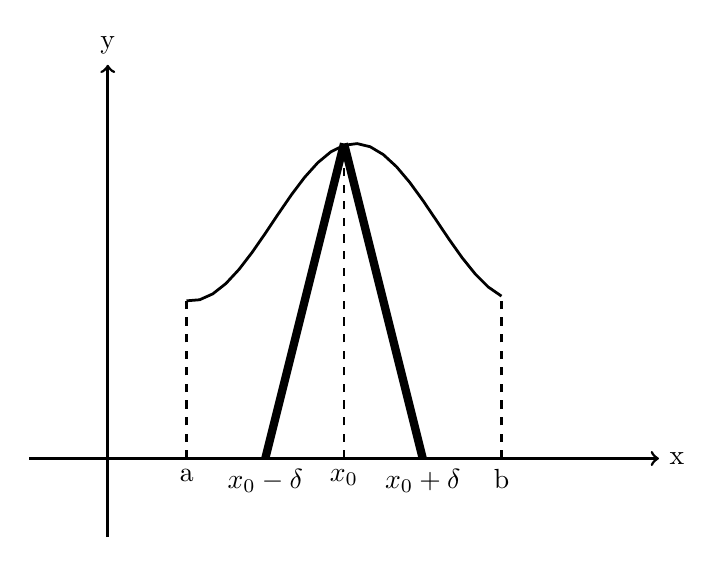
\begin{tikzpicture}[domain=1:5,line width=1pt]
\draw[->] (-1,0) -- (7,0);
\draw[->] (0,-1) -- (0,5);

\draw[style=dashed] (1,0) -- (1,2);
\draw[style=dashed] (5,0) -- (5,2);
\draw[style=dashed] (3,0) -- (3,4);

\draw[line width=3pt] (2,0) -- (3,4);
\draw[line width=3pt] (4,0) -- (3,4);

\node [right] at (7,0) {x};
\node [above] at (0,5) {y};

\draw plot (\x,{3-sin(\x*1.5 r)}) node[right] {};

\node [below] at (1,0) {a};
\node [below] at (2,0) {$x_0-\delta$};
\node [below] at (3,0) {$x_0$};
\node [below] at (4,0) {$x_0+\delta$};
\node [below] at (5,0) {b};
        
\end{tikzpicture}

$则\jf{a}{b}f(x)g(x)dx=\jf{x_0-\delta}{x_0+\delta}f(x)g(x)dx$

$=f(\zeta)\jf{x_0-\delta}{x_0+\delta}g(x)dx \ge \frac{f(x_0)}{2}$

$\nl$
$I=\jf{0}{1}\frac{ln(1+x)}{1+x^2}dx,令x=tgt,t\in [0,\frac{\pi}{4}]$

$=\jf{0}{\frac{\pi}{4}}ln(1+tgt)dt=\jf{0}{\frac{\pi}{4}}ln(1+\frac{sint}{cost})dt=\jf{0}{\frac{\pi}{4}}ln(\frac{sint+cost}{cost})dt$

$=\jf{0}{\frac{\pi}{4}}ln(\frac{cos(\frac{\pi}{2}-t)+cost}{cost})dt=\jf{0}{\frac{\pi}{4}}ln(\frac{2cos\frac{\pi}{4}cos(\frac{\pi}{4}-t)}{cost})dt$

$=\jf{0}{\frac{\pi}{4}}ln\sqrt 2dt+\jf{0}{\frac{\pi}{4}}lncos(\frac{\pi}{4}-t)dt-\jf{0}{\frac{\pi}{4}}lncostdt$

$令\frac{\pi}{4}-t=u,\jf{0}{\frac{\pi}{4}}lncosudu=-\jf{\frac{\pi}{4}}{0}lncosudu$

$原式=\jf{0}{\frac{\pi}{4}}ln\sqrt 2 dt$

$1.\jf{0}{a}f(x)dx=\jf{0}{a}f(a-x)dx$

$2.\jf{0}{\frac{\pi}{2}}f(sinx,cosx)dx=\jf{0}{\frac{\pi}{2}}f(cosx,sinx)dx$

$3. 若f(x)为周期T的函数,\jf{a}{a+T}f(x)dx=\jf{0}{T}f(x)dx$

$4.\jf{0}{\pi}xf(sinx)dx=\frac{\pi}{2}\jf{0}{\pi}f(sinx)dx,利用奇偶函数证明$

$\nl$

$I_1 = \jf{0}{\pi}(xsinx)^2dx,令I_2 = \jf{0}{\pi}(xcosx)^2dx,故I_1+I_2=\jf{0}{\pi}x^2dx,I_2-I_1=\jf{0}{\pi}x^2cos2xdx$

$\nl$

$\xtinf \frac{\jf{0}{x}|sint|dt}{x}$

$解:\forall k=1~n有\jf{0}{\pi}|sint|dt=\jf{(k-1)\pi}{k\pi}|sint|dt=\jf{0}{\pi}sintdt=2$

$\int arcsin \sqrt{\frac{x}{1+x}}dx,令t=arcsin\sqrt{\frac{x}{1+x}},则tg^2t=x,故I=tg^2t-\int tg^2tdt$

$\jf{0}{n\pi}|sint|dt=2n,设n\pi \le x< (n+1)\pi$

$\frac{2n}{(n+1)\pi}=\frac{\jf{0}{n\pi}|sint|dt}{(n+1)\pi} \le 原式 \le \frac{\jf{0}{(n+1)\pi}|sint|dt}{n\pi}=\frac{2(n+1)}{n\pi}$

$\nl$

$例:\jf{-\frac{\pi}{4}}{\frac{\pi}{4}}\frac{dx}{1+sinx},因为\jf{-a}{a}f(x)dx=\jf{0}{a}(f(x)+f(-x))dx$

$ 故原式 = \jf{0}{\frac{\pi}{4}}(\frac{1}{1+sinx}+\frac{1}{1-sinx})dx=2\jf{0}{\frac{\pi}{4}}dtgx=2tgx|_0^{\frac{\pi}{4}}$

$\nl$

$例:\jf{0}{\frac{\pi}{4}}\frac{1-sin2x}{1+sin2x}dx=\jf{0}{\frac{\pi}{4}}\frac{1-sin2(\frac{\pi}{4}-x)}{1+sin2(\frac{\pi}{4}-x)}dx=\jf{0}{\frac{\pi}{4}}\frac{1-cos2x}{1+cos2x}dx$

$=\jf{0}{\frac{\pi}{4}}tg^2xdx=\jf{0}{\frac{\pi}{4}}sec^2xdx-\jf{0}{\frac{\pi}{4}}dx=1-\frac{\pi}{4}$

$\nl$

$设f(x)=\jf{0}{a-x}e^{t(2a-t)}dt,求\jf{0}{a}f(x)dx$

$分析:f(a)=0,f'(x)=-e^{a^2-x^2}$

$\jf{0}{a}f(x)dx=xf(x)|_0^a-\jf{0}{a}xf'(x)dx=\jf{0}{a}xe^{a^2-x^2}dx=-\frac{1}{2}\jf{0}{a}e^{a^2-x^2}d(a^2-x^2)=\frac{e^{a^2}}{2}$

$证明:\jf{1}{a}f(x^2+\frac{a^2}{x^2})\frac{dx}{x}=\jf{1}{a}f(x+\frac{a^2}{x})\frac{dx}{x}$

$令x^2=t,则2xdx=dt$

$\jf{1}{a}f(x^2+\frac{a^2}{x^2})\frac{dx}{x}=\frac{1}{2}\jf{1}{a^2}f(t+\frac{a^2}{t})\frac{dt}{t}$

$=\frac{1}{2}[\jf{1}{a}f(t+\frac{a^2}{t})\frac{dt}{t}+\jf{a}{a^2}f(t+\frac{a^2}{t})\frac{dt}{t}]$

$在后一积分中令u=\frac{a^2}{t},则变为\jf{a}{1}f(t+\frac{a^2}{t})du(-\frac{1}{u^2}u)$

$\nl$

$f(x)=\jf{x}{x+1}sin(e^t)dt,证明e^x|f(x)| \le 2$

$令e^t=u,dt=\frac{1}{u}du,于是f(x)=\jf{e^x}{e^{x+1}}\frac{sinu}{u}du$

$f(x)=-\frac{cosu}{u}|_{e^x}^{e^{x+1}}-\jf{e^x}{e^{x+1}}\frac{cosu}{u^2}du=\frac{cose^x}{e^x}-\frac{cose^{x+1}}{e^{x+1}}-\jf{e^x}{e^{x+1}}\frac{cosu}{u^2}du$

$e^x|f(x)| \le |cose^x|+|\frac{cose^{x+1}}{e}|+(\jf{e^x}{e^{x+1}}\frac{cosu}{u^2}du)e^x$

$\le 1+\frac{1}{e}+(\jf{e^x}{e^{x+1}}\frac{1}{u^2}du)e^x=\frac{2}{e^x}e^x$

$例:证明\ntinf \jf{0}{\pi}|sinnx|ln(1+x)dx=\frac{2}{\pi}\jf{0}{\pi}ln(1+x)dx$

$分析:\jf{0}{\pi}|sinnx|ln(1+x)dx=\sum\limits_{k=1}^{n}\jf{\frac{k-1}{n}\pi}{\frac{k}{n}\pi}|sinnx|ln(1+x)dx$

$因为\jf{\frac{k-1}{n}\pi}{\frac{k}{n}\pi}|sinnx|dx,令nx=t,则有\jf{\frac{k-1}{n}\pi}{\frac{k}{n}\pi}|sint|\frac{t}{n}dt=\frac{1}{n}\jf{0}{\pi}sintdt=\frac{2}{n}$

$ln(1+x)在[0,+\infty)上递增,故有$

$\jf{\frac{k-1}{n}\pi}{\frac{k}{n}\pi}|sinnx|ln(1+x)dx \ge ln(1+\frac{k-1}{n}\pi)\jf{\frac{k-1}{n}\pi}{\frac{k}{n}\pi}|sinnx|dx=\frac{2}{n}ln(1+\frac{k-1}{n}\pi)$

$上式两边求和取极限$

$方法二:用积分中值定理$

$\jf{0}{\pi}|sinnx|ln(1+x)dx=\sum\limits_{k=1}^{n}\jf{\frac{k-1}{n}\pi}{\frac{k}{n}\pi}|sinnx|ln(1+x)dx$

$=\sum\limits_{k=1}^{n}ln(1+\zeta_k)\jf{\frac{k-1}{n}\pi}{\frac{k}{n}\pi}|sinnx|dx$

$=\sum\limits_{k=1}^{n}ln(1+\zeta_k)\frac{2}{n}$

$\nl$

$设f(x)在[0,+\infty)上单调递增,对\forall T>0,f(x) \in R[0,T]$

$证明:\xtinf f(x)=c的充要条件是\xtinf \frac{1}{x}\jf{0}{x}f(t)dt=c$

$必要性:要证\forall \epsilon >0,\exists X>0,|\frac{1}{x}\jf{0}{x}f(t)dt-c|<\epsilon,\forall x>X$

$因为\xtinf f(x)=c,\forall \epsilon >0,\exists x_0>0,c-\epsilon<f(x)<c+\epsilon,\forall x>x_0$

$\frac{1}{x}\jf{0}{x}f(t)dt=\frac{1}{x}\jf{0}{x_0}f(t)dt+\frac{1}{x}\jf{x_0}{x}f(t)dt$

$<无穷小量+\frac{1}{x}\jf{x_0}{x}(c+\epsilon)dt$

$=无穷小量+(c+\epsilon)(1-\frac{x_0}{x})$

$注意到f(x)\in R[0,x_0]故\frac{1}{x}\jf{0}{x_0}f(t)dt \to 0,(x \to \infty)$

$充分性须用到单调递增条件,否则存在反例:y=1+sinx$

$充分性:f(x)=\frac{1}{x}\jf{0}{x_0}f(x)dt \ge \frac{1}{x}\jf{0}{x_0}f(t)dt \to c,而f(x)=\frac{1}{x}\jf{x}{2x}f(x)dt \le \frac{1}{x}\jf{x}{2x}f(t)dt=2\frac{1}{2x}\jf{0}{2x}f(t)dt-\frac{1}{x}\jf{0}{x}f(t)dt \to 2c-c=c$

$\nl$

$例:设f(x)连续,\varphi (x)=\jf{0}{1}f(xt)dt,且\xtx{0}\frac{f(x)}{x}=A$

$讨论\varphi'(x)在x=0处的连续性$

$分析:f(0)=0,令xt=n,则\varphi (x)=\frac{1}{x} \jf{0}{x}f(u)du,x \ne 0$

$从而\varphi'(x)=\frac{xf(x)-\jf{0}{x}f(u)}{x^2}du,x \ne 0,另\varphi (0)=0$

$\varphi'(0)= \xtx{0} \frac{\varphi (x)-\varphi(0)}{x}=\xtx{0} \frac{\jf{0}{x}f(u)du}{x^2}=\xtx{0} \frac{f(x)}{2x}=\frac{A}{2}$

$\xtx{0} \varphi '(x)=\xtx{0} \frac{xf(x)-\jf{0}{x}f(u)du}{x^2} =\xtx{0}\frac{f(x)}{x}-\xtx{0}\frac{\jf{0}{x}f(u)du}{x^2}=A-\frac{A}{2}=\frac{A}{2}$

$故\varphi '(x)在x=0处连续$

$\nl$

$设f(x)在[a,b]上可导,f'(x)>0,f(x)>0,对图中所示面积A(x)B(x)$

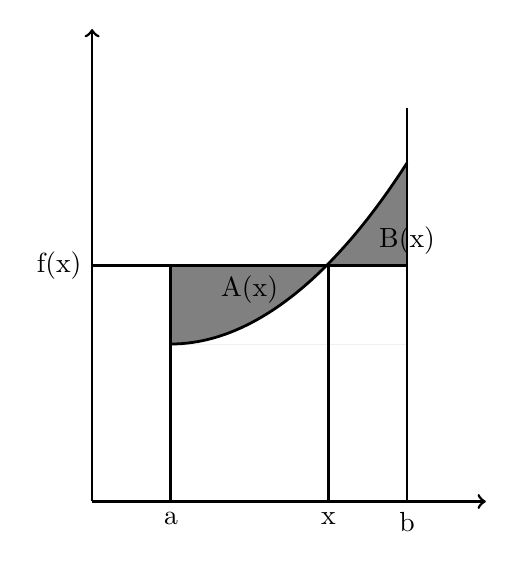
\begin{tikzpicture}[domain=1:5,line width=1pt]
\draw[->] (0,0) -- (5,0);
\draw[->] (0,0) -- (0,6);

\fill[gray] (4,2) -- (1,2) parabola (4,4.3);
\fill[white] (4,2) rectangle (1,3); 
\fill[gray] (1,3) -- (1,2) parabola (3,3);

\draw (1,2) parabola (4,4.3);

\draw (0,3) -- (4,3);

\draw (1,0) -- (1,3);
\draw (3,0) -- (3,3);
\draw (4,0) -- (4,5);
        
\node [below] at (2,3) {A(x)};
\node [above] at (4,3) {B(x)};
\node [below] at (1,0) {a};
\node [below] at (3,0) {x};
\node [below] at (4,0) {b};        
\node [left] at (0,3) {f(x)};        
\end{tikzpicture}

$证明:必存在x \in [a,b]使得\frac{A(x)}{B(x)}=1999$

$分析,A(x)=f(x)(x-a)-\jf{a}{x}f(t)dt=\jf{a}{x}(f(x)-f(t))dt$

$B(x)=\jf{x}{b}(f(t)-f(x))dt$

$可令F(x)=A(x)-1999B(x),验证F'(x)>0,验证F(a)<0,F(b)>0$

$\nl$

$设f(x)二阶可导,证明\exists \zeta_0 \in (a,b),使得\jf{a}{b}f(x)dx=(b-a)\frac{f(a)+f(b)}{2}-\frac{(b-a)^2}{12}f''(\zeta_0)$

$分析:试用分步积分法$

$\nl$

$设f(x) \in C[a,b],对\forall [\alpha,\beta] \subset [a,b]有$

$|\jf{\alpha}{\beta}f(x)dx| \le M(\beta - \alpha)^{1+\lambda},M>0,\lambda>0$

$证明:f(x)=0,\forall x \in [a,b]$

$(1)令F(x)=\jf{a}{x}f(t)dt,\forall x \in (a,b),取\Delta x使得x+\Delta x \in(a,b]$

$则|F(x+\Delta x)-F(x)|=|\jf{x}{x+\Delta x}f(t)dt| \le M \Delta x^{1+\lambda}$

$|\frac{F(x+\Delta x0-F(x)}{\Delta x}| \le M|\Delta x|^\lambda$

$f(x) \in C,|f(\zeta_x)| \le M|\Delta x|^\lambda,\zeta 介于x与x+\Delta x之间$

$当\Delta x \to,\zeta_x \to x,0 \le f(x) \le 0$

$(2)\forall x \in (a,b),有\{\epsilon_n\}(\epsilon_n > 0,\ntinf \epsilon_n=0)使得x+\epsilon_n \in [a,b]$

$则|\jf{x}{x+\epsilon_n}f(x)dx| \le M\epsilon_n^{1+\lambda}$

$x_n介于x与x+\epsilon_n,f(x_n)\epsilon_n=\jf{x}{x+\epsilon_n}f(x)dx \le M\epsilon_n^{1+\lambda}$

$\nl$

$设f''(x) \in c[0,1],f(0)=f(1)=0,且f(x) \ne 0 ,\forall x \in (0,1)$

$求证:\jf{0}{1}|\frac{f''(x)}{f(x)}|dx \ge 4$

$分析:设f(x)>0,\forall x \in (0,1),设maxf(x)=f(x_0)$

$故\exists x_1,x_2:f'(x_1)=\frac{f(x_0)}{x_0},f'(x_2)=-\frac{f(x_0)}{1-x_0}中值定理$

$从而有\jf{0}{1}|\frac{f''(x)}{f(x)}| \ge \frac{\jf{0}{1}|f''(x)|dx}{f(x_0)} \ge \frac{\jf{x_1}{x_2}|f''(x)|dx}{f(x_0)} \ge \frac{|\jf{x_1}{x_2}f''(x)dx|}{f(x_0)}$

$=\frac{1}{f(x_0)} |f'(x_2)-f'(x_1)| =\frac{1}{x_0(1-x_0)} \ge 4$

$\nl$

$f'(x) \in c[0,1], \jf{0}{1}f(x)dx=0,证明:\jf{0}{1}f^2(x)dx \le \jf{0}{1}[f'(x)]^2dx$

$(1)\exists x_1,x_2 \in (0,1],\jf{0}{1}fx(x)=f(x_1)=0,\jf{0}{1}f^2(x)dx=f^2(x_2)积分中值定理$

$利用Swharchz不等式,\jf{0}{1}f^2(x)dx=f^2(x_2)=(f(x_2)-f(x_1))^2$

$=(\jf{x_1}{x_2}f'(x)dx)^2 \le (\jf{x_1}{x_2}|f'(x)|dx)^2 \le (\jf{0}{1}|f'(x)|dx)^2$

$\le \jf{0}{1}dx \jf{0}{1}f'(x)^2dx = \jf{0}{1}f'(x)^2dx$

$(2)\exists \zeta \in [0,1]使得f(\zeta)=\jf{0}{1}f(x)dx=0$

$f^2(x)=[f(x)-f(\zeta)]^2=(\jf{\zeta}{x}f'(t)dt)^2$

$\le (\jf{\zeta}{x}f'(t)^2dt) (\jf{\zeta}{x}dt) \le \jf{0}{1}f'(x)^2dx$

$所以\jf{0}{1}f^2(x)dx \le \jf{0}{1}\{\jf{0}{1}f'(x)^2dx\}dx = \jf{0}{1}[f'(x)]^2dx$

$\nl$

$设f(x) \in c(a,b),\forall g(x) \in c[a,b],\jf{a}{b}f(x)g(x)dx=0(\jf{a}{b}g(x)dx=0)$

$证明f(x)必为常数$

$令g(x)=f(x)-\frac{1}{b-a}\jf{a}{b}f(x)dx,则\jf{a}{b}g(x)dx=0$

$因为\int kf(x) =k \int f(x) \to \jf{a}{b}(\frac{1}{b-a}\jf{a}{b}f(x)dx)g(x)dx=0$

$又因为\jf{a}{b}f(x)g(x)dx=0,$

$\jf{a}{b}g(x)f(x)-(\frac{1}{b-a}\jf{a}{b}f(x)dx)g(x)=0$

$故有等价于\jf{a}{b}g^2(x)dx=0,故g(x)=0$

$故f(x)=\frac{1}{b-a}\jf{a}{b}f(x)dx=c$

$\nl$

$例:集合F是满足下列条件的实函数f (1)f(x) \in c[0,1]且非负$

$(2)f(0+0,f(1)=1$

$证明:inf_F \{\jf{0}{1}f(x)dx\}=0,F=\{x^n\},并问是否存在\varphi \in F:\jf{0}{1}\varphi(x)dx=0$

$\nl$

$例:设f(x) \in c[a,b],\jf{a}{b}x^nf(x)dx=0,n=0,1,2,3..n,$

$证明:f(x)在(a,b)内至少有n+1个零点$

$考虑n=1时,因为\jf{a}{b}f(x)dx=0,故f(x)在[a,b]内至少有一个零点$

$设为f(x_0)=0,若只有一个零点x_0,则f(x)在x_0两边异号$

$故f(x)(x-x_0)在[a,b]内同号,故\jf{a}{b}f(x)(x-x_0)dx \ne 0,与$

$\jf{a}{b}f(x)xdx=0 -x_0 \jf{a}{b}f(x)=0矛盾$

$\nl$

$设正值函数f(x)\in C(R),以\frac{\pi}{2}为周期,又$

$\jf{0}{\frac{\pi}{2}}e^{f(x)}ln[f(x)]sinxdx=\jf{0}{\frac{\pi}{2}}e^{f(x)}ln[f(x)]cosxdx=0$

$证明:f(x)在(0,\pi)内至少存在四个点,使得f(x_i)=1$

\end{document}

